% !BIB program = bibtex
% !TeX root = ../main.tex

\chapter{Problem Formulation}

In this chapter, we will introduce the scenario of the carpooling fairness problem. Then formulate the problem into a mathematical model with given parameters and decision variables.

\section{Problem Description}

The object of this research is to minimize the maximum percentage of cost saving when a passenger chooses to carpool, with consideration of the number of drivers, car capacity and routing limit constraints.

Take Figure 3-1 as an example scenario; Passenger 1 and Passenger 2 are requesting a trip. When Passenger 1 chooses to take a ride by himself/herself, called "exclusive" riding shown as Figure 3-2, it would cost \$5. We can describe the scenario as a shortest path problem from $S$ to $D_1$, and $P_1$ is a must-pass node. We use Steiner tree to solve this kind of shortest path problem with must-pass nodes. Passenger 2's "exclusive" riding would also cost \$5 in Figure 3-3. In this case, it would be a shortest path problem from $S$ to $D_2$ with $P_2$ as a must-pass node.

When the passengers choose to take a carpool, which is called "sharing" riding. We can describe the scenario as a shortest problem from $S$ to $D_1$ with $P_1$, $P_2$ and $D_2$ as must-pass nodes or $S$ to $D_2$ with $P_1$, $P_2$ and $D_1$ as must-pass nodes. In Figure 3-4 is one of the best case, which would cost \$8 for all the passengers, in Figure 3-5 would cost the same \$8 and both of the fares they could share are \$5 ( $\overline{P_2D_1}$ and $\overline{P_2D_2}$ respectively); however, in Figure 3-4 would cost $\overset{\overline{P_1P_2}}{1} + \frac{1}{2} \times \overset{\overline{P_2D_1}}{5} = \$3.5$ for Passenger 1 and $\frac{1}{2} \times \overset{\overline{P_2D_1}}{5} + \overset{\overline{D_1D_2}}{1} = \$3.5$ for Passenger 2, in Figure 3-5 would cost $\overset{\overline{P_1P_2}}{1} + \frac{1}{2} \times \overset{\overline{P_2D_2}}{5} + \overset{\overline{D_2D_1}}{1} = \$4.5$ for Passenger 1 and $\frac{1}{2} \times \overset{\overline{P_2D_2}}{5} = \$2.5$ for Passenger 2.

\begin{figure}[htp]
  \centering
  \captionsetup{justification=centering}
  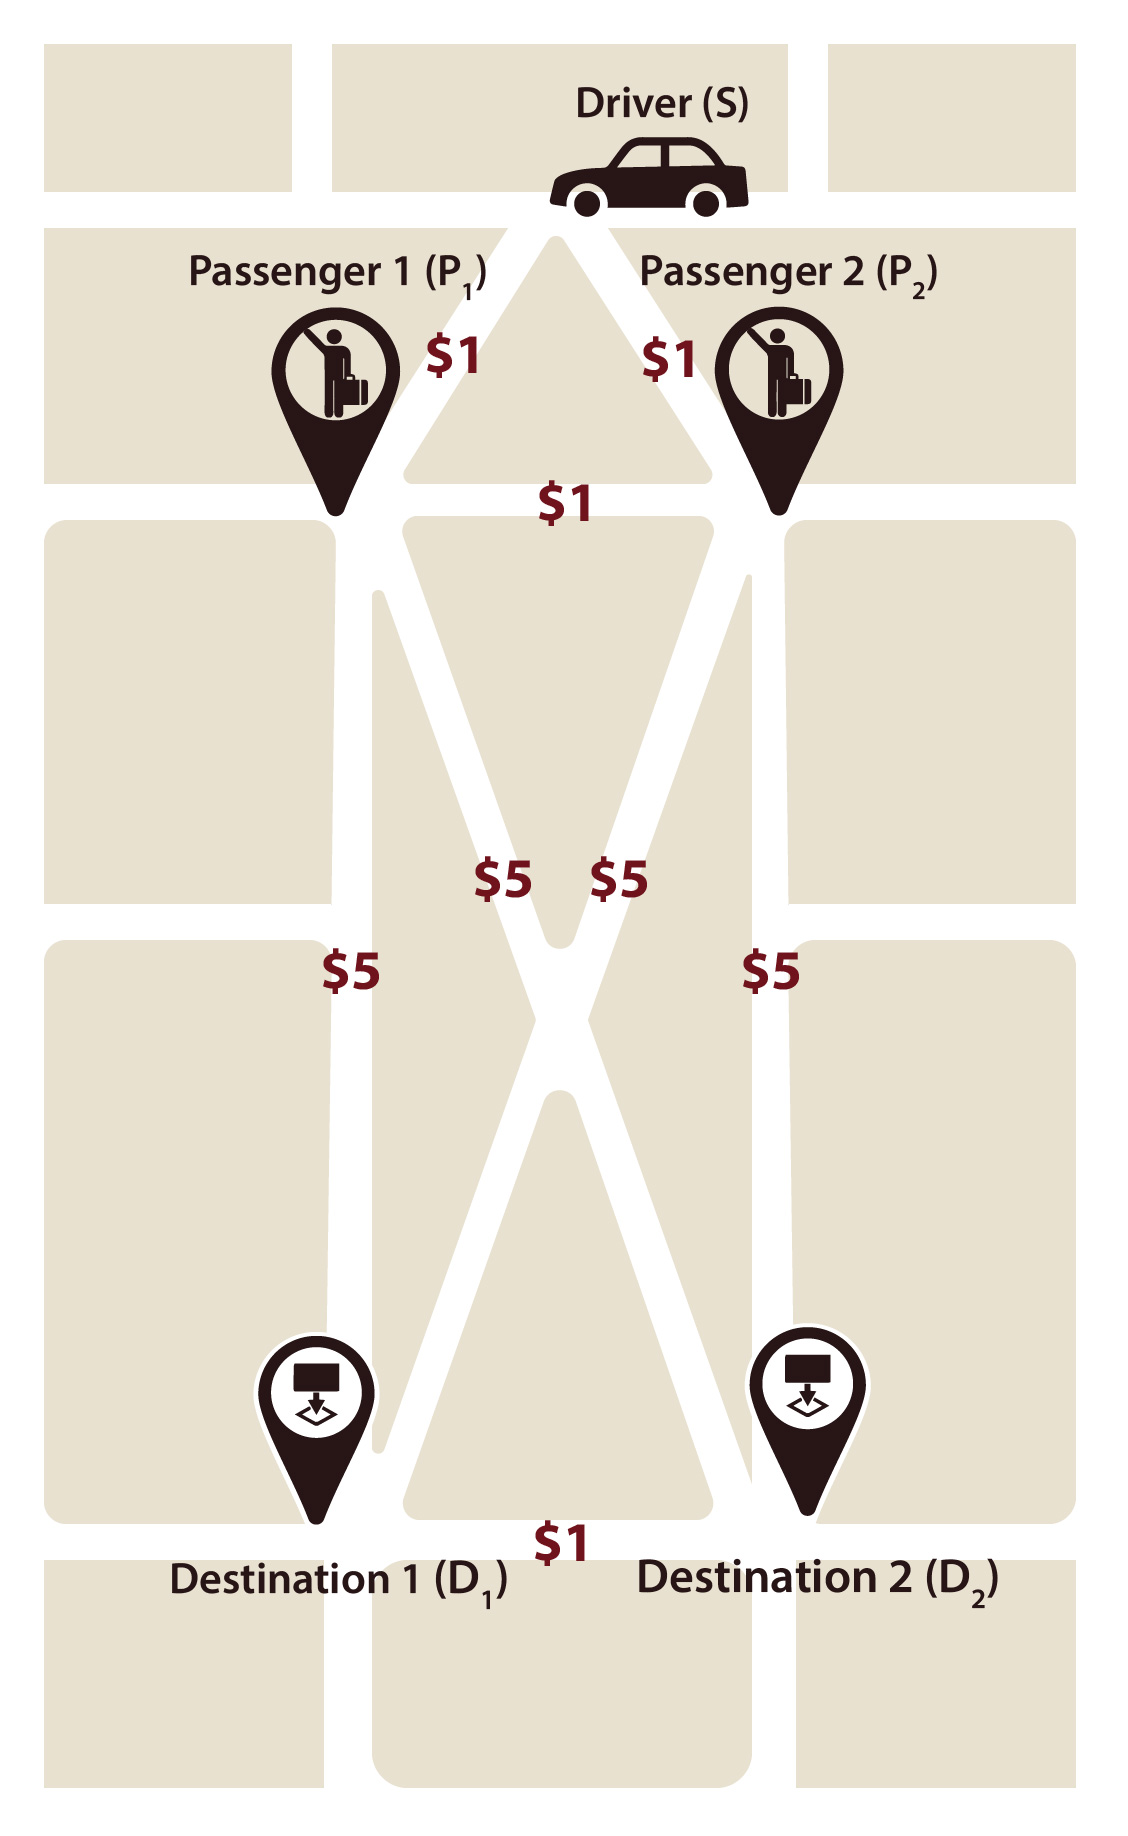
\includegraphics[width=6cm]{figures/mapV2.jpg}
  \caption{Example road network with driving fare and points of passengers and their destinations}
\end{figure}

\begin{figure}[htp]
  \centering
  \captionsetup{justification=centering}
  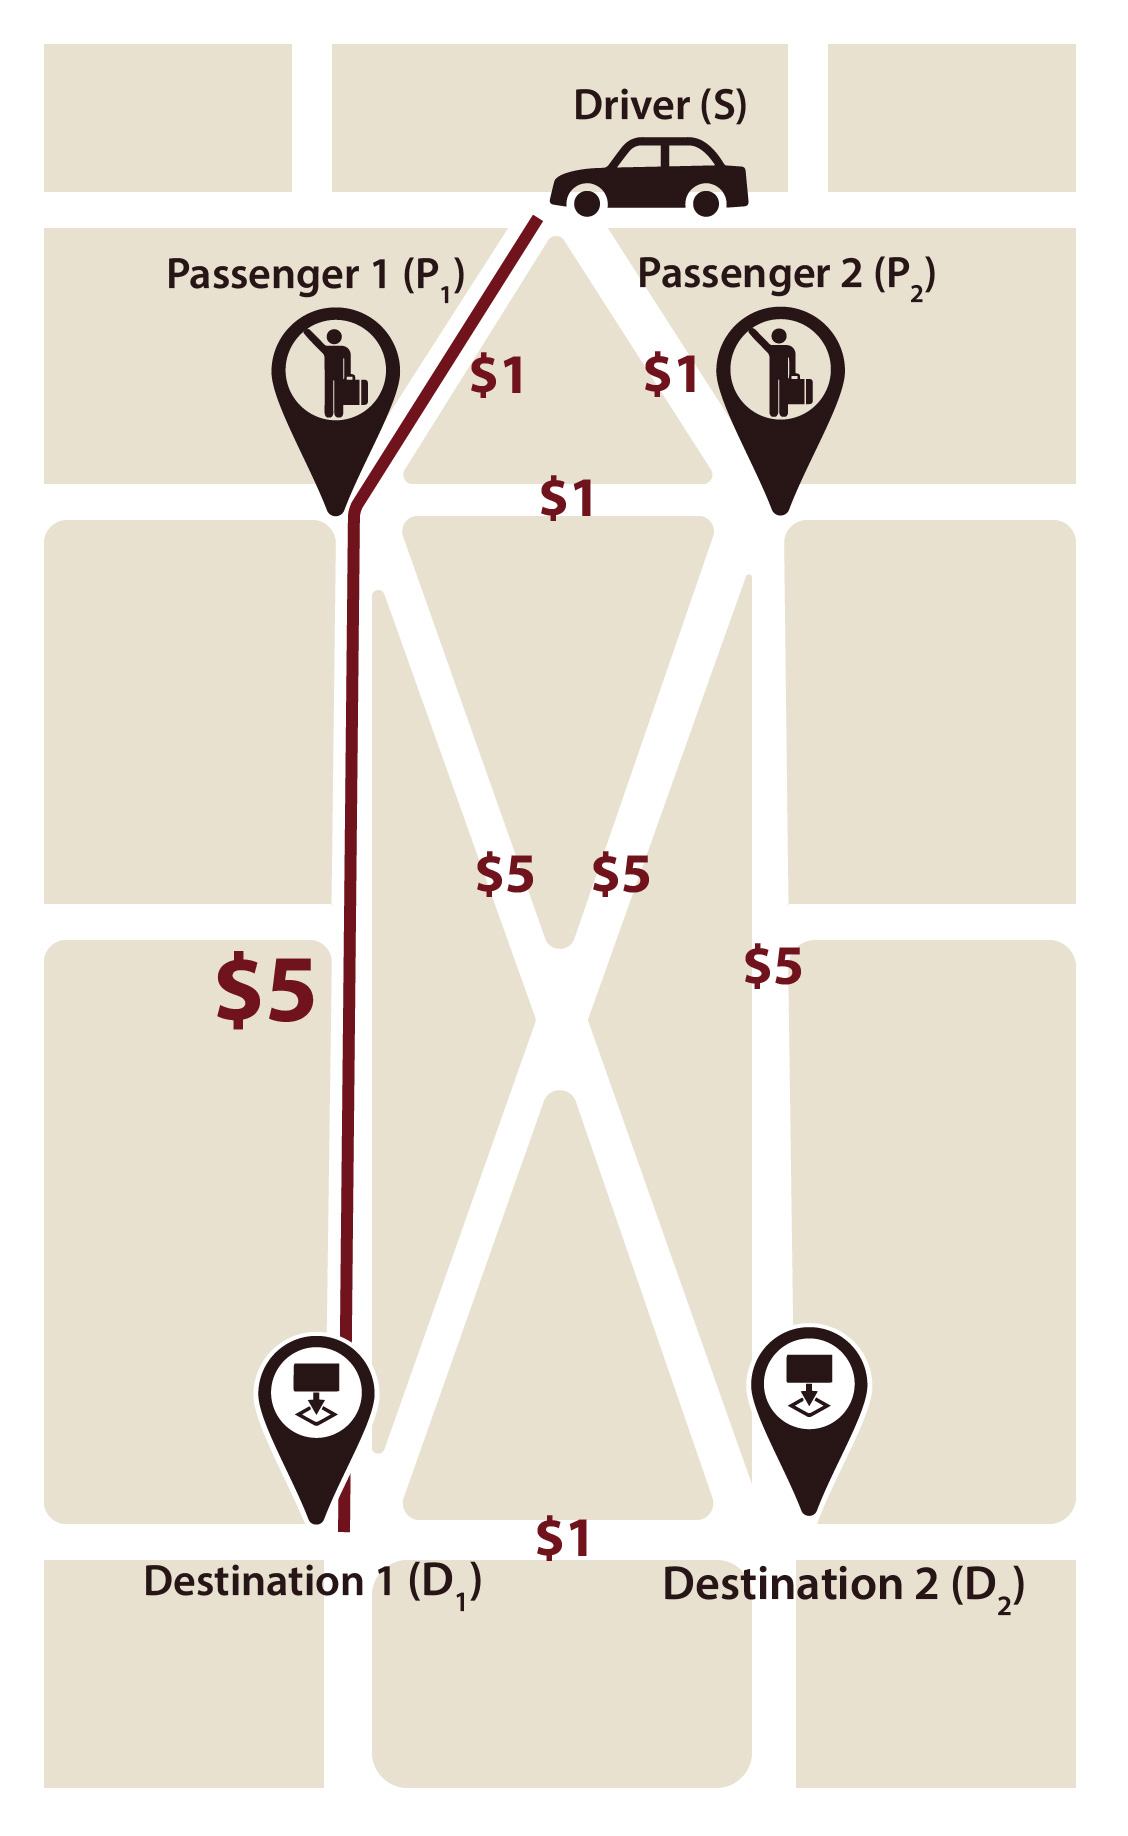
\includegraphics[width=6cm]{figures/mapV2_1.jpg}
  \caption{Best routing path when the driver only serving Passenger 1}
\end{figure}

\begin{figure}[htp]
  \centering
  \captionsetup{justification=centering}
  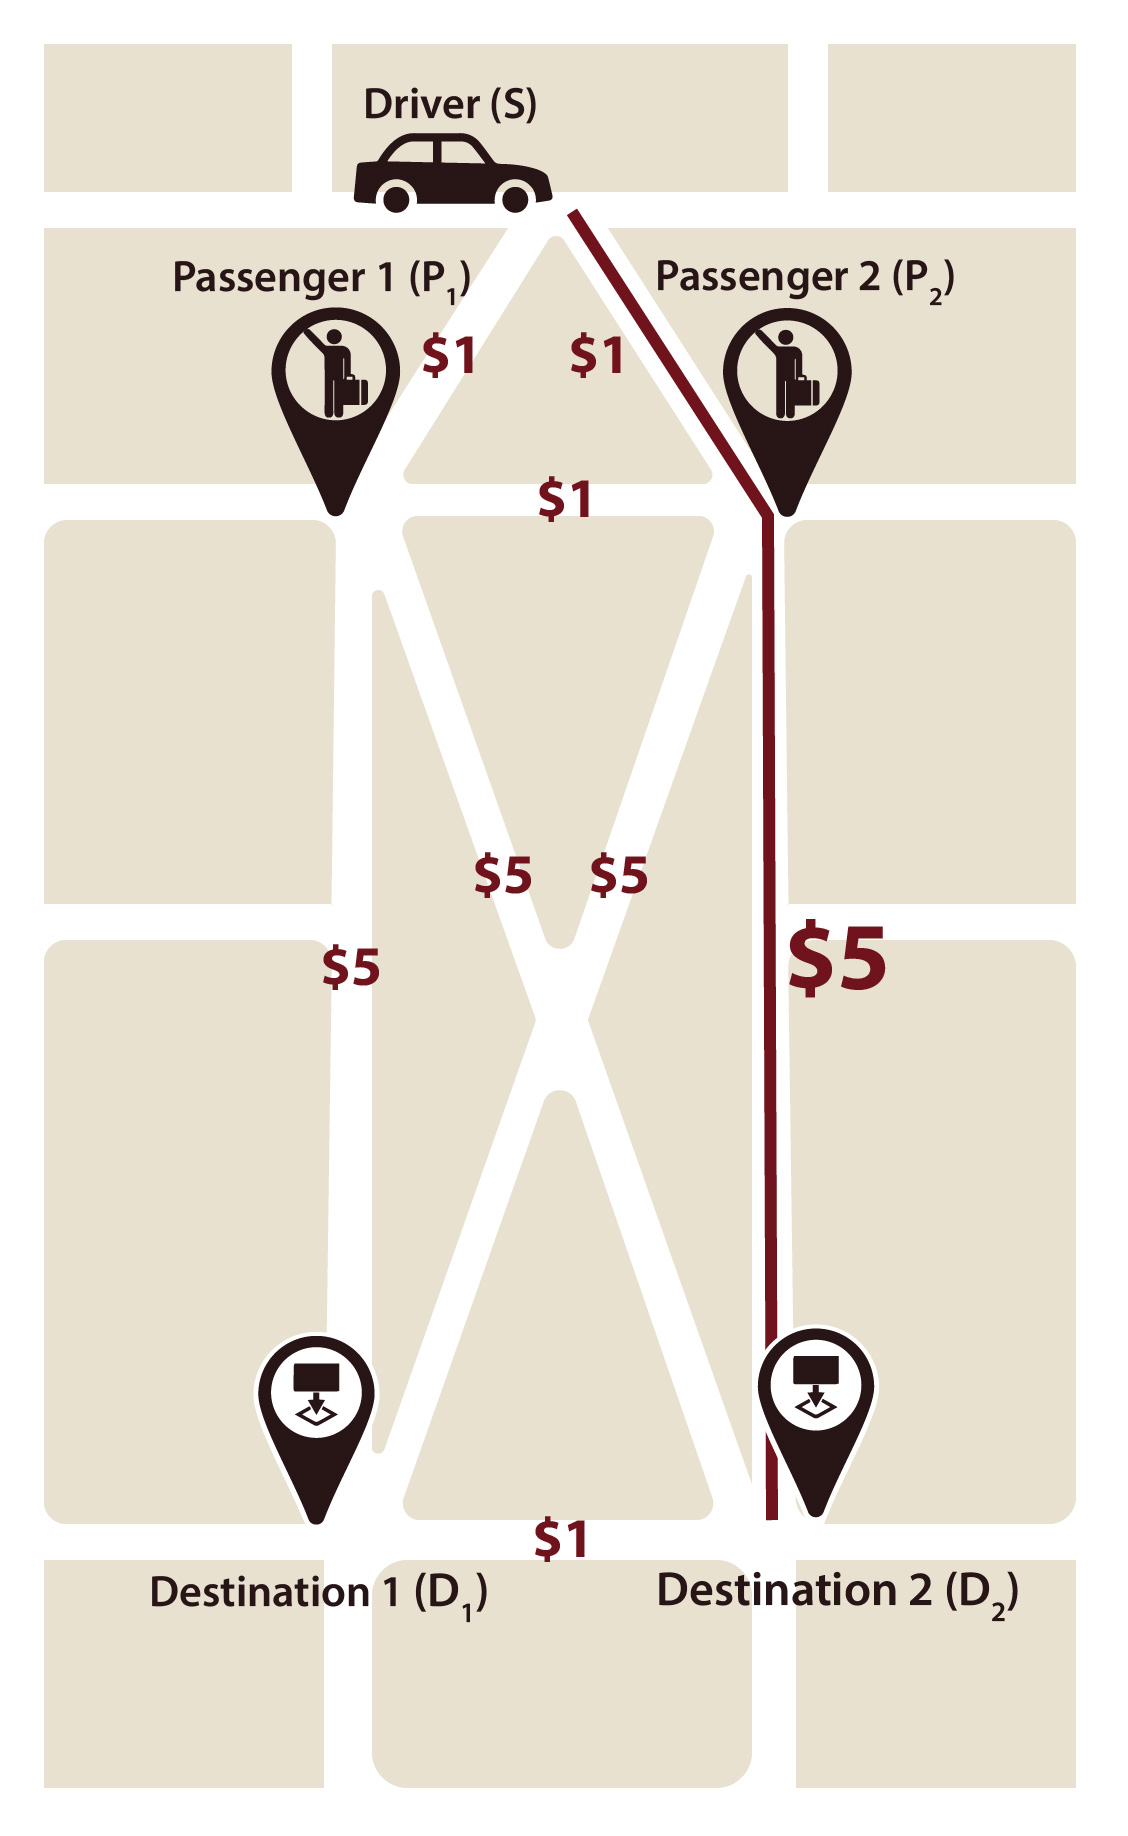
\includegraphics[width=6cm]{figures/mapV2_4.jpg}
  \caption{Best routing path when the driver only serving Passenger 2}
\end{figure}

\begin{figure}[htp]
  \centering
  \captionsetup{justification=centering}
  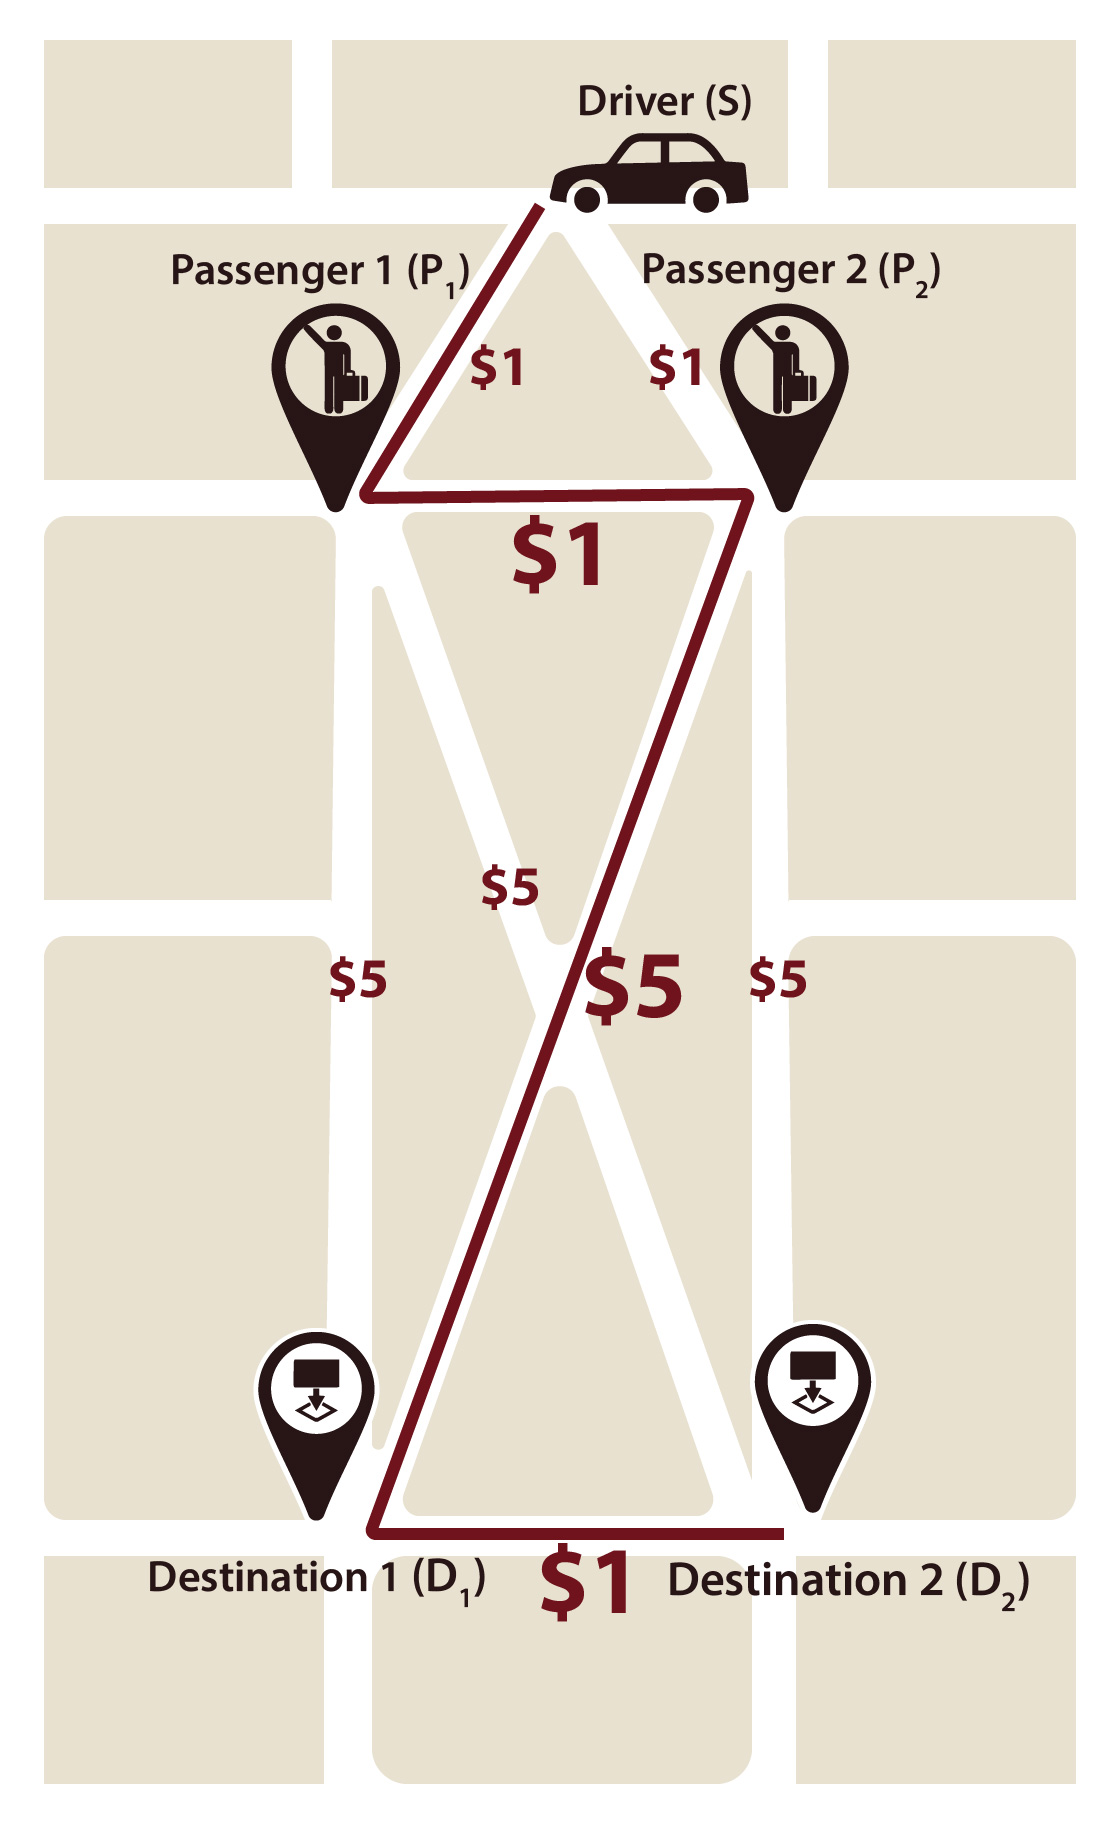
\includegraphics[width=6cm]{figures/mapV2_2.jpg}
  \caption{One of the best routing when both Passenger 1 and Passenger 2 carpool}
\end{figure}

\begin{figure}[htp]
  \centering
  \captionsetup{justification=centering}
  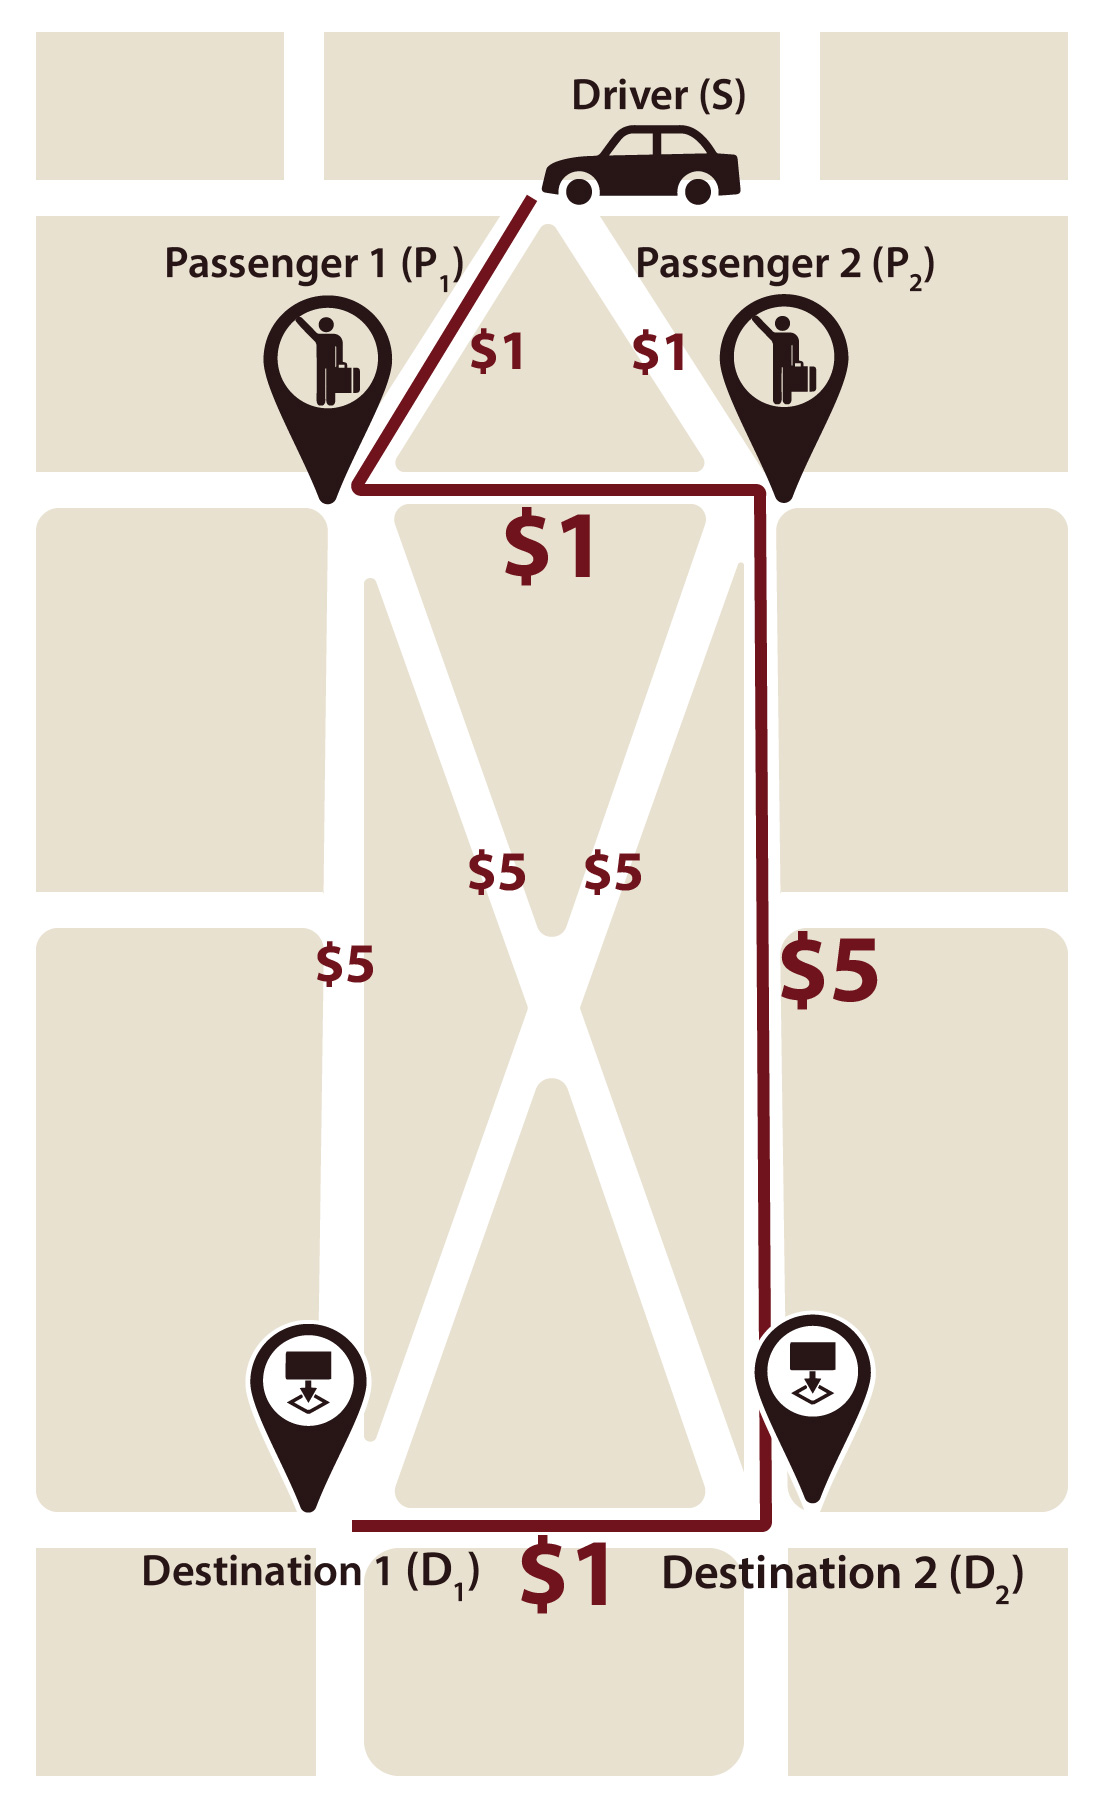
\includegraphics[width=6cm]{figures/mapV2_3.jpg}
  \caption{Another best routing when both Passenger 1 and Passenger 2 carpool}
\end{figure}
\newpage

\subsection{Assumptions}

There are three assumption in out system:

\begin{enumerate}
  \item System calculation time is not considered, that is, assume that drivers' location will still keep unchanged after the time of system calculation.
  \item The carpooling fare is shared equally by the time passengers in the vehicle. For a specific link in the route with $n$ passengers, the fare of the link for a passenger will be divided by $n$.
  \item Length of any link is proportional to the fare rate on the link.
  \item All the passengers on the trip will accept the offer of carpooling.
  \item Total driving time is equal to sum of time spending of links that pass by.
 \end{enumerate}

\subsection{Fairness of Vehicle Dispatching}

In order to consider the fairness when dispatching driver, we introduce Jain's fairness index to avoid unfair situation:

$Firness\ Index = f_A(x) = \frac{\left(\sum\limits_{i=1}^{n} x_i\right)^2}{n \sum\limits_{i=1}^{n} x_i^2}$

We take accumulate driving requests that a driver has received as the metrics for fairness. That is, when a driver receives more driving requests in the past, he/she should give his/her chance of receiving a new driving request to the one who takes fewer driving requests.

As a new driving request comes, we need to ensure our system must get more or at least keep the same fairness. Hence, we form a constraint that the fairness index can not decrease compared to the previous fairness index.

However, when the driving resource changes, such as a new driver joins our system, it will violate our constraint for fairness. Because the newcomer has not taken any driving request before, the fairness will decrease. Even if a driver leaves our system, the fairness will increase or decrease due to the driver's situation. As a result, we need to reset the fairness index to the initial state and reset all the drivers' accumulated driving requests to 0. Nevertheless, it will make the fairness index's denominator to 0, which can not be divided. To avoid this situation, we assign a virtual driver with one accumulated driving request, which will make the fairness index to $\frac{1}{(n+1)}$, where $n$ is the number of drivers in our system. Moreover, for any situation that the fairness index will decrease when dispatching a new driving request, the fairness will reset.

\newpage

\section{Mathematical Model}

We will go through the detailed given parameters and decision variables in the mathematical model before describing our mathematical model.

The road network is represented as a weighted graph $G = (N, L)$, where $N$ is the nodes and $L$ is the links in the graph.

\renewcommand\arraystretch{1.5}
\par
\begin{table}[ht]
  \centering
  \caption{Notations of given parameters}
  \begin{tabularx}{\textwidth}{cX}
  \toprule
  Notation & Description \\
  \midrule
    $R$ & Set of riding requests (take $i$ as index) \\
    $C$ & Set of cab drivers in the system \\
    $L$ & Set of links on the road network \\
    $N$ & Set of nodes on the road network \\
    $o_i$ & Origin node of riding request $i \in R$, $o_i \in N$ \\
    $d_i$ & Destination node of riding request $i \in R$, $o_i \in N$ \\
    $q_i$ & Number of passengers associates with riding request $i \in R$ \\
    $s_i$ & Maximum passengers limit of carpooling associates with riding request $i \in R$ \\
    $T_i$ & Maximum waiting time of riding request $i \in R$. \\
    $Q_c$ & Maximum load capacity for driver, $c \in C$ \\
    $l_{o_i}$ & Artificial link of node $o_i$ \\
    $l_{d_i}$ & Artificial link of node $d_i$ \\
    $P_{co_i}$ & Set of paths from current location of driver $c \in C$ to origin node of riding request $i \in R$ \\
    $P_{cd_i}$ & Set of paths from current location of driver $c \in C$ to destination node of riding request $i \in R$ \\
    $P_c$ & Set of available paths for driver $c \in C$  \\
    $t_{cl}$ & The driving time for driver $c \in C$ on the link $l \in L$ \\
    $f_{cl}$ & The fare rate for driver $c \in C$ on the link $l \in L$ \\
    $f_{ci}$ & The fare rate of exclusive riding request $i \in R$ for driver $c \in C$ \\
    $B_c$ & Set of riding requests that driver $c \in C$ has picked up \\
  \bottomrule
  \end{tabularx}
\end{table}  
\par

\renewcommand\arraystretch{1.5}
\par
\begin{table}[ht]
  \centering
  \caption{Notations of given parameters}
  \begin{tabularx}{\textwidth}{cX}
  \toprule
  Notation & Description \\
  \midrule
    $E$ & Maximum detour ratio for hitchhiking \\
    $\delta_{pl}$ & Indicator function which is 1 if link $l \in L$ on the route $p \in P_c \cup P_{co_i} \cup P_{cd_i}$ \\
    $a_r$ & Total fare that the driver $r \in R$ has earned before current decision round. \\
    $\alpha$ & The fairness index in the previous decision round. \\
  \bottomrule
  \end{tabularx}
\end{table}  
\par

\begin{table}[ht]
  \centering
  \caption{Notations of decision variables}
  \begin{tabularx}{\textwidth}{cX}
  \toprule
  Notation & Description \\
  \midrule
    $x_{p}$ & Binary variable, 1 if route $p \in P_{co_i}$ is chosen for driver $c \in C$; 0 otherwise. \\
    $y_{p}$ & Binary variable, 1 if route $p \in P_{cd_i}$ is chosen for driver $c \in C$; 0 otherwise. \\
    $z_{p}$ & Binary variable, 1 if route $p \in P_c$ is chosen for driver $c \in C$; 0 otherwise. \\
    $w_{ci}$ & Binary variable, 1 if riding request $i \in R$ is chosen for driver $c \in C$; 0 otherwise. \\
    $u_{li}$ & Binary variable, 1 if artificial link $l \in l_{o_i}, i \in R$ is assigned to any drivers; 0 otherwise. \\
    $v_{li}$ & Binary variable, 1 if artificial link $l \in l_{d_i}, i \in R$ is assigned to any drivers; 0 otherwise. \\
  \bottomrule
  \end{tabularx}
\end{table}  
\newpage

\subsubsection*{Objective Function}

The objective function is to maximize the minimum discount percentage when applying carpooling among passengers in one trip.

\begin{align*}
  \max_{i \in R} \min_{c \in C} \frac{w_{ci} f_{ci} - carpool\ cost_c}{w_{ci} f_{ci}} \tag{IP1} \\
\end{align*}

\subsubsection*{Constraints}

\begin{align}
  \intertext{Constraint \eqref{waiting_time} ensures the waiting time is suit for the riding request.}
  & \sum\limits_{p \in P_{co_i}} x_{p} \delta_{pl} t_{cl} \leq T_i && \forall l \in L, c \in C, i \in R \label{waiting_time} \\
  \intertext{Constraints \eqref{path_limit_origin}, \eqref{path_limit_destination}, \eqref{path_limit} ensure there is only one path selected for a driver.}
  & \sum\limits_{p \in P_{co_i}} x_{p} \leq 1 && \forall c \in C, i \in R \label{path_limit_origin} \\
  & \sum\limits_{p \in P_{cd_i}} y_{p} \leq 1 && \forall c \in C, i \in R \label{path_limit_destination} \\
  & \sum\limits_{p \in P_{c}} z_{p} \leq 1 && \forall c \in C \label{path_limit} \\
  \intertext{Constraint \eqref{riding_request_limit} ensures a riding request will only be assigned by one driver.}
  & \sum\limits_{c \in C} w_{ci} \leq 1 && \forall i \in R \label{riding_request_limit}
  \intertext{Constraint \eqref{pick_up_drop_off_limit} ensures a riding request will be picked up before dropping off.}
  & \sum\limits_{p \in P_{co_i}} x_{p} \delta_{pl} f_{cl} \leq \sum\limits_{p \in P_{cd_i}} y_{p} \delta_{pl} f_{cl} && \forall l \in L, c \in C, i \in R \label{pick_up_drop_off_limit} \\
  \intertext{Constraints \eqref{link_limit_origin}, \eqref{link_limit_destination} ensure artificial links will be passed by if the order associates with the link is assigned.}
  & \sum\limits_{c \in C} w_{ci} = u_{li} && \forall l \in L, i \in R \label{link_limit_origin} \\
  & \sum\limits_{c \in C} w_{ci} = v_{li} && \forall l \in L, i \in R \label{link_limit_destination} \\
  \intertext{Constraint 3.2 ensures the selected link on the route we chose is on the shortest path.}
  & \sum\limits_{p \in P_r} x_p \delta_{pl} \leq u_l && \forall l \in L \\
  \intertext{Constraint 3.4 ensures that all the routes to passengers or destinations we chose is on the shortest path and overlap the route we chose.}
  & \sum\limits_{p \in P_w} z_p \delta_{pl} \leq u_l && \forall w \in W \\
  \intertext{Constraint 3.7 ensures the fairness index after current decision round will not less than the previous decision round.}
  & \frac{\left(\sum\limits_{r \in R} b_r\right)^2}{\sum\limits_{r \in R} 1 \sum\limits_{r \in R} b_r^2} \geq \alpha \\
  \intertext{Constraint 3.8 is the fairness index in the previous decision round.}
  & \frac{\left(\sum\limits_{r \in R} a_r\right)^2}{\sum\limits_{r \in R} 1 \sum\limits_{r \in R} a_r^2} \leq \alpha \\
  \intertext{Constraint 3.9 ensures there is only one driver selected for a passenger.}
  & \sum\limits_{r \in R} v_{cr} \leq 1
\end{align}
